\documentclass[a4paper,12pt,singlespacing]{article}

\usepackage{titlesec}
\usepackage{setspace}
\usepackage[utf8]{inputenc}
\usepackage{graphicx}
\usepackage{color}
\usepackage[hidelinks]{hyperref}
\usepackage[style=ieee, sorting=none]{biblatex}
\usepackage[english]{babel}
\usepackage{tikz}
\usetikzlibrary{positioning, fit, calc, shapes, arrows.meta}
\usepackage{booktabs}
\usepackage{pgfplots}
\usepackage{amssymb}
\usepackage{pifont}
\usepackage{float}
\usepackage{listings,xcolor}
\usepackage[table]{xcolor}
\usepackage{caption}
\usepackage{tocloft}
\usepackage{tikz}
\usepackage{float}
\usepackage{etoolbox}
\usepackage{pdflscape}
\usepackage[acronym]{glossaries}
\makeglossaries
\addbibresource{sample.bib}

\titlespacing*{\section}{0pt}{35pt}{35pt}
\titlespacing*{\subsection}{0pt}{20pt}{20pt}
\titlespacing*{\subsubsection}{0pt}{10pt}{10pt}

\usepackage[automark,headsepline]{scrlayer-scrpage}
\pagestyle{scrheadings}
\automark{subsection}
\ihead{\headmark}
\ohead{\pagemark}
\newcommand{\cmark}{\textcolor{green!60!black}{\ding{51}}}
\newcommand{\xmark}{\textcolor{red!80!black}{\ding{55}}}  

\lstdefinestyle{cppstyle}{
	language=c,
	numbers=left,
	numberstyle=\footnotesize,
	numbersep=6pt,
	breaklines=true,
	showstringspaces=false,
	basicstyle=\ttfamily\footnotesize,
	keywordstyle=\bfseries\color[rgb]{0,0,1},
	commentstyle=\color{gray},
	stringstyle=\color{red},
	frame=single,
	rulecolor=\color{black}
}

\begin{document}
\selectlanguage{english}

\setlength{\parindent}{0ex}

\begin{titlepage}
	
	%----------------------------------------------------------------------------------------
	%	LOGO SECTION
	%----------------------------------------------------------------------------------------
	
	\begin{minipage}{0.4\textwidth}
		\begin{flushleft} \large
			
\includegraphics[width=3.5cm]{./Images/conti_logo.png}
		\end{flushleft}
	\end{minipage}
	~
	\begin{minipage}{0.5\textwidth}
		\begin{flushright} \large
			
\includegraphics[width=7cm]{./Images/logo.png}
		\end{flushright}
	\end{minipage}\\[1.5cm]
	
	%----------------------------------------------------------------------------------------
	
	\newcommand{\HRule}{\rule{\linewidth}{0.5mm}} % Defines a new command for the horizontal lines, change thickness here
	
	\center % Center everything on the page
	
	%----------------------------------------------------------------------------------------
	%	HEADING SECTIONS
	%----------------------------------------------------------------------------------------
	
	\textsc{\LARGE Ravensburg Weingarten University}\\[1cm] % Name of your university/college
	\textsc{\large  \textbf{Bachelor Thesis}}\\[0.5cm] % Minor heading such as course title
	
	%----------------------------------------------------------------------------------------
	%	TITLE SECTION
	%----------------------------------------------------------------------------------------
	
	\HRule \\[0.4cm]
	{ \huge \bfseries Developing a Concept for Automated Testing of IPC Middleware – Demonstrated with eCAL}\\[0.4cm] % Title of your document
	\HRule \\[1.5cm]
	
	%----------------------------------------------------------------------------------------
	%	AUTHOR SECTION
	%----------------------------------------------------------------------------------------
	\hspace*{0.40cm}
	\begin{minipage}{0.5\textwidth}
		\begin{flushleft}\fontsize{11pt}{14pt}\selectfont
			\textbf{Author:} Emircan Tutar\\[4pt]
			\textbf{Address:} Heyderstr. 7\\[4pt]
			\textbf{City:} 88131 Lindau\\[7pt]
			\textbf{Student ID:} 35606\\[4pt]
			\textbf{Program:} Applied Computer Science\\[4pt]
		\end{flushleft}
	\end{minipage}
	~
	\begin{minipage}{0.43\textwidth}
		\begin{flushleft} \fontsize{11pt}{14pt}\selectfont
			\textbf{1st Supervisor:} \\[2pt]
			Prof. Dr. Marius Hofmeister \\
			Ravensburg Weingarten University \\[10pt]
			\textbf{2nd Supervisor:} \\[2pt]
			M.Sc. Kerstin Keller \\
			Continental\\[7pt]
		\end{flushleft}
	\end{minipage}\\[2cm]
	
	%----------------------------------------------------------------------------------------
	%	DATE SECTION
	%----------------------------------------------------------------------------------------
	
	{\large \today}\\[0cm] % Date, change the \today to a set date if you want to be precise
	
	\vfill % Fill the rest of the page with whitespace
	
	
\end{titlepage}
\pagestyle{plain}
\pagenumbering{roman}
\pagebreak
\vspace*{2cm}
\textbf{Modern software development is characterized by the need for rapid adaptation to evolving requirements. Distributed systems, where components run on separate computing nodes and communicate via defined interfaces, are central to many domains, including automation, robotics, and embedded systems. To enable seamless communication between these components, inter-process communication (IPC) frameworks are widely used. These frameworks facilitate efficient and reliable data exchange, which is essential for the flexible implementation of new features and system updates.} \\

\textbf{As distributed systems become more complex, ensuring their reliability and functional correctness becomes increasingly important. Communication failures or unexpected interactions between components can have critical consequences, particularly in safety-relevant fields. Therefore, a central challenge emerges: how can the correctness and robustness of IPC-based systems be systematically validated through testing? This thesis addresses this challenge by developing a structured testing concept to the specific demands of IPC middleware environments.} \\

\textbf{To this end, established testing methodologies including integration, and system-level tests are analyzed and adapted for distributed IPC systems. The emphasis is placed on creating maintainable and reusable test structures that support long-term system evolution. The developed concepts will be demonstrated and evaluated using a practical implementation, ensuring their applicability to real-world middleware systems.}

\pagebreak
% Abstand
\setlength{\cftbeforesecskip}{10pt}
\setlength{\cftbeforesubsecskip}{6pt}
\setlength{\cftbeforesubsubsecskip}{2pt}

% Einrückung & Breite
\setlength{\cftsecindent}{0pt}
\setlength{\cftsubsecindent}{20pt}
\setlength{\cftsubsubsecindent}{40pt}

% Schriftarten
\renewcommand{\cftsecfont}{\normalsize\bfseries}
\renewcommand{\cftsubsecfont}{\normalsize}
\renewcommand{\cftsubsubsecfont}{\small}

\renewcommand{\cftsecpagefont}{\bfseries}
\renewcommand{\cftsubsecpagefont}{\normalfont}
\renewcommand{\cftsubsubsecpagefont}{\normalfont}
\tableofcontents
\pagebreak

% List of Figures
\begingroup
\setlength{\baselineskip}{1.3\baselineskip}
\listoffigures
\endgroup
\phantomsection
\addcontentsline{toc}{section}{List of Figures}
\pagebreak


% List of Listings
\renewcommand{\lstlistlistingname}{List of Listings}
\begingroup
\setlength{\baselineskip}{1.3\baselineskip}
\lstlistoflistings
\endgroup
\phantomsection
\addcontentsline{toc}{section}{List of Listings}
\pagebreak


\section*{List of Abbreviations}
\phantomsection
\addcontentsline{toc}{section}{List of Abbreviations}

\begin{tabbing}
	XXXXXXXXX \= XXXXXXXXXXXXXXXXXXXXXXXXXXX \kill % length
	\textbf{API} \> Application Programming Interface\\[0.3cm]
	\textbf{BDD} \> Behavior-Driven Development\\[0.3cm]
	\textbf{CD} \> Continuous Delivery\\[0.3cm]
	\textbf{CI} \> Continuous Integration\\[0.3cm]
	\textbf{CI/CD} \> Continuous Integration / Continuous Delivery\\[0.3cm]
	\textbf{CLI} \> Command Line Interface\\[0.3cm]
	\textbf{DDS} \> Data Distribution Service\\[0.3cm]
	\textbf{eCAL} \> enhanced Communication Abstraction Layer\\[0.3cm]
	\textbf{IPC} \> Inter-Process Communication\\[0.3cm]
	\textbf{IoT} \> Internet of Things\\[0.3cm]
	\textbf{N:1} \> Many-to-One Communication Pattern\\[0.3cm]
	\textbf{1:N} \> One-to-Many Communication Pattern\\[0.3cm]
	\textbf{N:N} \> Many-to-Many Communication Pattern\\[0.3cm]
	\textbf{PID} \> Process Identifier\\[0.3cm]
	\textbf{QoS} \> Quality of Service\\[0.3cm]
	\textbf{RPC} \> Remote Procedure Call\\[0.3cm]
	\textbf{ROS} \> Robot Operating System\\[0.3cm]
	\textbf{SH} \> Shell Script\\[0.3cm]
	\textbf{SHM} \> Shared Memory\\[0.3cm]
	\textbf{TCP} \> Transmission Control Protocol\\[0.3cm]
	\textbf{UAT} \> User Acceptance Testing\\[0.3cm]
	\textbf{UDP} \> User Datagram Protocol\\[0.3cm]
\end{tabbing}

\pagebreak
\pagenumbering{arabic}
\pagestyle{scrheadings}

\selectlanguage{english}
\clearpage

\section{Introduction}

This chapter introduces the overall topic and scope of the thesis. Section 1.1 outlines the motivation for developing a structured testing approach for IPC  middleware. Section 1.2 defines the main objectives of the thesis, and Section 1.3 provides an overview of its structure.

\subsection{Motivation}

Inter-process communication (IPC) middleware plays a critical role in modern distributed systems. It enables software components (often running on different machines) to exchange data efficiently, coordinate actions, and maintain system coherence. This is especially important in domains such as robotics, automotive systems, and the Industrial Internet of Things (IIoT), where real-time requirements and fault tolerance are essential \cite{coulouris2012}.

\vspace{1em}
Despite the increasing reliance on IPC middleware, systematic and reusable testing concepts for these technologies are still lacking in many projects. While unit tests verify individual components in isolation, they are not sufficient for ensuring the correctness of interactions between distributed nodes, especially in failure-prone or time-sensitive environments.

\vspace{1em}
Middleware frameworks such as ROS 2 and DDS have introduced their own tools and mechanisms to support system-level validation e.g., in ROS 2  \texttt{launch\_testing} \cite{ros2_launch_testing}, or monitoring utilities in DDS implementations like eProsima Fast DDS and RTI Connext DDS \cite{eprosima_fast_dds, rti_connext_dds}. However, these approaches are often tightly coupled to the specifics of the respective middleware architectures and cannot be directly transferred to other systems.

\vspace{1em}
The enhanced Communication Abstraction Layer (eCAL) is a IPC framework designed for fast, scalable communication across processes and hosts \cite{ecal_github}. Although it provides a flexible communication model, eCAL currently lacks a standardized strategy for testing at the system level. While some components are covered by unit or functional tests, there is no unified infrastructure for evaluating end-to-end communication, message integrity under stress, or failure handling in realistic scenarios.

\vspace{1em}
This thesis addresses that gap by developing a generic testing concept for IPC middleware and applying it concretely to the case of eCAL.

\subsection{Objective}

The goal of this thesis is to develop and evaluate a testing concept that enables structured and automated validation of inter-process communication (IPC) middleware. A particular focus lies on the design of a reusable system-level testing methodology that can be adapted to different middleware architectures. As a practical example, the concept will be implemented and demonstrated using the eCAL framework.

\vspace{1em}
The core objectives are:

\begin{itemize}
	\item Design a structured testing approach for conducting system tests of IPC middleware in distributed environments.
	\item Investigate suitable tools, frameworks, and technologies for implementing automated tests.
	\item Apply the developed testing concept to eCAL and validate its applicability through representative test scenarios.
\end{itemize}

\subsection{Outline}

The structure of this thesis is as follows:

\begin{itemize}
	\item \textbf{Chapter 2: Theoretical Foundations}:  Introduces testing principles and discusses core concepts of inter-process communication and middleware.
	\item \textbf{Chapter 3: Test Requirements for IPC Middleware}: Identifies key requirements for a testing strategy in IPC systems.
	\item \textbf{Chapter 4: Tool Evaluation and Selection}: Evaluates potential tools and frameworks for implementing the test system.
	\item \textbf{Chapter 5: Design and Automation of Tests}: Describes the test architecture and implementation of selected test cases.
	\item \textbf{Chapter 6: Conclusion and Outlook}: Summarizes the findings.
\end{itemize}








\selectlanguage{english}
\clearpage
\section{Theoretical Foundations}

In this chapter, the theoretical background necessary to understand the development of a system testing framework for eCAL is presented. Section 2.1 introduces essential concepts in software testing, such as test levels, types, and techniques. Section 2.2 explains the concept of distributed systems, including their characteristics and common use cases. Section 2.3 provides the fundamentals of inter-process communication (IPC) and highlights different communication mechanisms. In Section 2.4, the role of middleware in distributed environments is discussed, with a focus on commonly used solutions such as ROS, DDS, and eCAL. Finally, Section 2.5 outlines specific challenges in testing middleware systems, presents current testing approaches, and analyzes the limitations of testing practices in the context of eCAL.

\subsection{Software Testing Fundamentals}

Software testing is a structured process aimed at verifying that software meets the defined requirements and performs reliably in its intended environment. This section introduces the core concepts of software testing, including test levels, test types, test techniques, and the test pyramid.

\subsubsection{Test Levels}

Software testing is organized into different levels to detect defects at specific stages of development. According to Ammann and Offutt \cite{ammann2016introduction}, the main test levels are:

\vspace{1em}
\textbf{Unit Testing:}

\vspace{0.4em}
Unit testing focuses on verifying individual components or units of a system in isolation. These tests are typically written and executed by developers during the coding phase and aim to detect logic errors or incorrect function outputs early \cite{pressman2014software}.

\vspace{1em}
\textbf{Integration Testing:}

\vspace{0.4em}
Integration testing validates the interaction between different modules or components. This level ensures that data is correctly passed and interpreted between integrated parts of the application \cite{burnstein2003practical}.

\newpage

\textbf{System Testing:}

\vspace{0.4em}
System testing examines the entire integrated system as a whole. It verifies that the system behaves correctly under various conditions, including performance, security, and usability aspects \cite{myers2011art}.

\vspace{1em}
In distributed systems, however, the boundary between integration testing and system testing can become blurred. Since individual components often run on different machines or communicate asynchronously, validating their interaction frequently involves testing parts of the overall system behavior as well. As a result, what is formally considered integration testing may already include system-level characteristics such as network latency, synchronization, or fault tolerance.

\vspace{1em}
\textbf{Acceptance Testing:}

\vspace{0.4em}
Acceptance testing, also called User Acceptance Testing (UAT), determines whether the software fulfills the business requirements and is ready for deployment. It is usually performed by end users or stakeholders \cite{kaner1999testing}.
\vspace{0.2em}

\subsubsection{Test Types}

There are two major types of tests commonly used in software quality assurance:

\vspace{1em}
\textbf{A) Functional Testing}

\vspace{0.4em}
Functional testing ensures that software features behave according to their specifications. It is typically performed through techniques like equivalence class partitioning and boundary value analysis \cite{pressman2014software}.

\vspace{1em}
\textbf{B) Non-functional Testing}

\vspace{0.4em}
Non-functional testing addresses aspects such as performance, reliability, maintainability, and usability. These qualities are essential for a software product to function effectively in production environments \cite{kaner1999testing}.

\vspace{0.4em}
\subsubsection{Test Techniques}

Various techniques are used to design efficient and targeted test cases:

\vspace{1em}
\textbf{Black-Box Testing}

\vspace{0.4em}
Black-box testing validates the system's functionality without considering its internal code structure. Testers use input-output analysis to confirm expected behavior \cite{myers2011art}.

\vspace{1em}
\textbf{White-Box Testing}

\vspace{0.4em}
White-box testing is based on knowledge of the internal structure and logic of the system. Testers examine decision paths, loops, and control structures to ensure code coverage \cite{burnstein2003practical}.

\vspace{1em}
\textbf{Gray-Box Testing}

\vspace{0.4em}
Gray-box testing combines elements of black-box and white-box approaches. It requires partial knowledge of the internal workings to create more targeted and effective test cases \cite{ammann2016introduction}.

\subsubsection{Test Pyramid}

The test pyramid is a widely recognized concept used to structure testing strategies in a scalable and maintainable way. It was introduced by Mike Cohn \cite{cohn2009succeeding} to help development teams allocate their testing efforts effectively across different levels of abstraction.

\begin{figure}[H]
	\centering
	\begin{tikzpicture}[scale=1.6]
		
		% Bottom Layer: Unit Tests
		\fill[green!40] (0,0) -- (8,0) -- (6.5,1.7) -- (1.5,1.7) -- cycle;
		
		% Middle Layer: Integration Tests
		\fill[yellow!40] (1.5,1.7) -- (6.5,1.7) -- (5.2,3.3) -- (2.8,3.3) -- cycle;
		
		% Top Layer: UI Tests
		\fill[red!40] (2.8,3.3) -- (5.2,3.3) -- (4,4.8) -- cycle;
		
		
		% Labels
		\node at (4,1) {\textbf{Unit Tests}};
		\node at (4,2.5) {\textbf{Integration Tests}};
		\node at (4,3.8) {\shortstack{\textbf{UI/}\\\textbf{End-to-End}\\\textbf{Tests}}};
		
		% Title
		\node[font=\bfseries] at (4,5.3) {Test Pyramid};
		
	\end{tikzpicture}
	\caption{The Test Pyramid illustrating test distribution across levels}
	\label{fig:testpyramid}
\end{figure}

At the base of the pyramid lies a large number of unit tests. These are fast, automated, and verify individual components or functions in isolation. Unit tests provide immediate feedback during development and help detect issues early, making them the foundation of efficient software testing.

\vspace{1em}
The middle layer consists of fewer integration tests. These tests check how different modules or components interact with each other and help uncover interface-related defects that are not visible during unit testing.

\vspace{1em}
At the top of the pyramid are the end-to-end or UI tests. These are high-level tests that simulate real user interactions across the entire system. Although essential for validating system behavior from a user perspective, they are typically slower, more fragile, and more expensive to maintain.

\vspace{1em}
As visualized in Figure~\ref{fig:testpyramid}, the pyramid illustrates the principle that lower-level tests should be more numerous and faster, while higher-level tests should be fewer and more focused. This structure promotes reliable, maintainable, and cost-effective testing workflows.

\subsection{Distributed Systems}

\subsubsection{Definition and Concepts}

A distributed system is a network of independent computers that appears to users as a single coherent system. In distributed systems, multiple computing devices communicate and coordinate their activities by passing messages to achieve a common goal \cite{tanenbaum2017}. Such systems consist of independent components located on different networked computers, which interact with each other by exchanging messages.

\vspace{1em}
The primary goal of distributed systems is to share resources, increase performance, and provide reliable and fault-tolerant operations. Resources such as processing power, memory, storage, and data can be shared between multiple nodes within the system, enhancing system efficiency and scalability \cite{coulouris2012}.

\vspace{1em}
Figure~\ref{fig:distributed_architecture} illustrates a basic distributed system consisting of multiple independent nodes communicating over a network. Each node may serve a specific role, such as providing services, accessing shared resources, or coordinating tasks.

\begin{figure}[H]
	\centering
	\begin{tikzpicture}[
		node/.style={draw, thick, minimum width=2.8cm, minimum height=1cm, rounded corners=5pt, fill=blue!10},
		conn/.style={->, thick},
		network/.style={draw, fill=gray!10, rounded corners=2pt}
		]
		
		% Nodes
		\node[node] (client1) at (-4, 2) {Client Node A};
		\node[node] (client2) at (4, 2) {Client Node B};
		\node[node] (server1) at (-2, 0) {Service Node A};
		\node[node] (server2) at (2, 0) {Service Node B};
		
		% Network Cloud
		\node[network, minimum width=5cm, minimum height=1.2cm] (network) at (0,-2) {Network};
		
		% Arrows from Clients to Services
		\draw[conn] (client1) -- (server1);
		\draw[conn] (client2) -- (server2);
		
		% Arrows from Services to Network
		\draw[conn] (server1) -- (network);
		\draw[conn] (server2) -- (network);
		
	\end{tikzpicture}
	\caption{Basic architecture of a distributed system with multiple clients and services connected through a network}
	\label{fig:distributed_architecture}
\end{figure}


\subsubsection{Characteristics and Challenges}

Distributed systems have several key characteristics, including concurrency, scalability, transparency, and fault tolerance. Concurrency refers to multiple processes executing simultaneously. Scalability describes the capability of the system to grow easily in size and workload. Transparency ensures the complexity of the system remains hidden from users, providing an impression of a single unified system. Fault tolerance describes the system's capability to continue operation even when individual components fail \cite{tanenbaum2017}.

\vspace{1em}
However, developing and managing distributed systems can be challenging. Problems related to communication delays, synchronization between processes, security, and managing the complexity of the overall system must be addressed effectively to ensure reliable operations \cite{coulouris2012}.

\subsubsection{Application Areas}

Distributed systems are widely used across many industries. In automotive systems, they support advanced driver-assistance systems (ADAS), autonomous driving, and vehicle communication systems. Robotics heavily relies on distributed systems for complex coordination tasks, such as collaborative robotics, autonomous navigation, and real-time control. The Internet of Things (IoT) is another prominent application area, where distributed systems enable efficient communication between countless smart devices and sensors, facilitating smart homes, smart cities, and industrial automation \cite{tanenbaum2017,coulouris2012}.



\subsection{Inter-Process Communication (IPC)}

\subsubsection{Overview and Importance}

Inter-process communication (IPC) refers to mechanisms that allow processes to communicate and exchange data. IPC is a crucial component in distributed and concurrent systems, enabling different software processes running on one or multiple computers to coordinate and share information effectively \cite{stallings2018}. Effective IPC mechanisms are essential for ensuring the smooth and reliable functioning of complex software systems, especially in critical applications such as automotive control systems, robotics, and industrial automation \cite{tanenbaum2015}.

\subsubsection{Common IPC Mechanisms}

There are several commonly used IPC mechanisms, each suitable for different scenarios and requirements. The most frequently used methods include shared memory, message passing, and remote procedure calls (RPC) \cite{stallings2018,tanenbaum2015}.

\begin{figure}[H]
	\centering
	\begin{tikzpicture}[
		node/.style={draw, thick, minimum width=3.5cm, minimum height=1cm, rounded corners=5pt, fill=blue!10},
		conn/.style={->, thick},
		label/.style={font=\bfseries, align=center}
		]
		
		% Shared Memory
		\node[label] at (0,8) {Shared Memory};
		\node[node] (shmA) at (-3,7) {Process A};
		\node[node] (shmB) at (-3,5.5) {Process B};
		\node[draw, fill=gray!20, minimum width=2.5cm, minimum height=1.5cm, rounded corners=4pt] at (4,6.25) (shm) {Shared Memory};
		\draw[conn] (shmA) -- (shm);
		\draw[conn] (shmB) -- (shm);
		
		% Message Passing
		\node[label] at (0,4.3) {Message Passing};
		\node[node] (msgA) at (-3,3.3) {Process A};
		\node[node] (msgB) at (4,3.3) {Process B};
		\draw[conn] (msgA) -- node[above] {Message} (msgB);
		
		% RPC
		\node[label] at (0,1.3) {Remote Procedure Call (RPC)};
		\node[node] (rpcClient) at (-3,0.3) {Client Process};
		\node[node] (rpcServer) at (4,0.3) {Server Process};
		\draw[conn] (rpcClient) -- node[above] {RPC Call} (rpcServer);
		\draw[conn] (rpcServer) -- node[below] {Result} (rpcClient);
		
	\end{tikzpicture}
	\caption{Comparison of common IPC mechanisms: Shared Memory, Message Passing, and Remote Procedure Call (RPC)}
	\label{fig:ipc_methods}
\end{figure}


\vspace{1em}
\newpage
Figure~\ref{fig:ipc_methods} illustrates a simplified comparison of common IPC mechanisms. Shared memory allows processes to access a common memory region directly. Message passing transfers data through explicit send/receive actions. RPC abstracts communication by allowing a process to call functions in another process as if they were local.

\vspace{1em}
\textbf{Shared Memory:}

Shared memory is one of the fastest IPC methods, allowing processes to communicate directly by accessing a common area of memory. Processes write and read data directly into this shared space, avoiding the overhead of explicit communication. However, managing synchronization and ensuring data integrity can become challenging and requires careful implementation of synchronization methods, such as semaphores or mutexes \cite{stallings2018, ipc_performance_analysis}.

\vspace{1em}
\textbf{Message Passing:}

\vspace{0.4em}
Message passing involves processes communicating through messages. This approach ensures a clear separation between processes, providing safer communication. Messages are sent explicitly from one process to another using defined communication channels, such as pipes or sockets. While message passing typically has higher overhead compared to shared memory, it is easier to manage synchronization, and it allows better scalability in distributed environments \cite{tanenbaum2015}.

\vspace{1em}
\textbf{Remote Procedure Calls (RPC):}

\vspace{0.4em}
Remote Procedure Calls enable processes to invoke procedures or functions on remote systems as if they were local calls. RPC abstracts network communication, making distributed system interactions easier to develop and maintain. RPC is widely used in distributed applications and middleware solutions due to its simplicity and clear programming model, despite some performance overhead from serialization and network transmission \cite{coulouris2012}.

\subsubsection{Zero-Copy Communication}

Zero-copy communication is an advanced IPC technique designed to minimize unnecessary data copying between processes. Traditional communication methods often involve copying data multiple times, significantly reducing performance and increasing latency. Zero-copy mechanisms avoid this overhead by allowing direct data transfers between processes, usually through shared memory. By reducing the data copies, zero-copy enhances performance and efficiency in systems with high throughput and low latency requirements, such as high-performance computing or real-time systems \cite{raiciu2017}.



\subsection{Middleware in Distributed Systems}

While IPC mechanisms define how processes communicate, middleware abstract these and provide a structured interface for distributed applications.

\subsubsection{Definition and Role of Middleware}

Middleware is software that sits between applications and the underlying operating system or network infrastructure, enabling easier communication and coordination within distributed systems. Its main role is to simplify development by abstracting complexities associated with networked and distributed computing, such as communication protocols, data exchange, and interoperability between diverse systems \cite{bernstein1996}. Middleware allows software developers to focus more on the application logic rather than the low-level communication and network details.

\subsubsection{Common Middleware Solutions}

Various middleware technologies are available today, each designed to address specific communication and coordination needs. Some widely used middleware solutions include the Robot Operating System (ROS) \cite{quigley2009}, the Data Distribution Service (DDS) \cite{pardo2003}, and the enhanced Communication Abstraction Layer (eCAL) \cite{ecal_official_docs}.

\vspace{1em}
Table~\ref{tab:middleware_comparison} presents a layered architecture comparison between ROS, DDS, and eCAL. Each middleware abstracts the communication stack differently, but all provide core functionality for distributed system communication.

\begin{table}[H]
	\centering
	\renewcommand{\arraystretch}{1.20}
	\begin{tabular}{|p{2.25cm}|p{3.22cm}|p{3.22cm}|p{3.22cm}|}
		\hline
		\textbf{Layer} & \textbf{ROS} & \textbf{DDS} & \textbf{eCAL} \\
		\hline
		Application Layer & User Applications & User Applications & User Applications \\
		\hline
		Middleware API & rospy, roscpp & DDS API & eCAL API (C++, Python, etc.) \\
		\hline
		Core-Components & ROS-Master, Topics, Services & RTPS Protocol & Pub/Sub, RPC \\
		\hline
		Transport Layer & TCP-ROS, UDP-ROS & UDP/IP & Shared-Memory, UDP, TCP \\
		\hline
		Operating System & Linux, Windows, macOS & OS-dependent & Linux, Windows, macOS \\
		\hline
	\end{tabular}
	\caption{Architecture comparison between ROS, DDS, and eCAL middleware}
	\label{tab:middleware_comparison}
\end{table}

\vspace{1em}
\textbf{Robot Operating System (ROS):}
\vspace{0.4em}

ROS is an open-source middleware widely used in robotics. It provides a structured communication framework that includes services like message passing, data visualization, hardware abstraction, and numerous tools for robotics development. ROS simplifies building complex robotic systems by offering standardized communication interfaces and extensive community-supported tools and libraries \cite{quigley2009}.

\vspace{1em}
\textbf{Data Distribution Service (DDS):}
\vspace{0.4em}

DDS is a standardized middleware designed primarily for real-time and high-performance distributed applications. It employs a publisher-subscriber communication model, where components communicate by exchanging messages without direct connections between producers and consumers. DDS provides reliable and scalable communication, making it suitable for critical applications such as automotive systems, aerospace, industrial automation, and healthcare \cite{pardo2003}.

\vspace{1em}
\textbf{Enhanced Communication Abstraction Layer (eCAL):}
\vspace{0.4em}

\textbf{Overview and Architecture}
\vspace{0.4em}

The enhanced Communication Abstraction Layer (eCAL) is an open-source middleware designed specifically for efficient inter-process communication (IPC) in distributed environments. It simplifies the exchange of data between processes running on the same device or across multiple networked computers. eCAL uses a decentralized publish-subscribe architecture, allowing multiple processes to communicate directly without relying on a central broker \cite{ecal_github}.

\vspace{1em}
eCAL has a modular and flexible architecture. It supports multiple transport layers, including shared memory for communication between processes on the same machine and TCP or UDP for communication over networks. This adaptive approach ensures optimal performance by automatically selecting the best available communication method based on the system's environment and requirements \cite{ecal_official_docs}.

\vspace{1em}
Figure~\ref{fig:ecal_architecture} illustrates the basic eCAL architecture. It shows how multiple publisher and subscriber nodes communicate over topics. Additionally, a monitoring component observes the activity of each node to support debugging and analysis.
\\
\begin{figure}[H]
	\centering
	\begin{tikzpicture}[
		component/.style={draw, thick, minimum width=3cm, minimum height=1cm, rounded corners=5pt, fill=blue!10},
		arrow/.style={->, thick}
		]
		
		% Nodes
		\node[component] (pub1) at (0,2.5) {Publisher Node A};
		\node[component] (pub2) at (-2,1) {Publisher Node B};
		\node[component] (sub1) at (6,2.5) {Subscriber Node A};
		\node[component] (sub2) at (8,1) {Subscriber Node B};
		\node[component, fill=orange!15] (monitor) at (3,-1) {eCAL Monitoring Tool};
		
		% Arrows
		\draw[arrow] (pub1) -- node[above] {Topic 1} (sub1);
		\draw[arrow] (pub2) -- node[below] {Topic 2} (sub2);
		\draw[arrow, dashed] (pub1) -- (monitor);
		\draw[arrow, dashed] (pub2) -- (monitor);
		\draw[arrow, dashed] (sub1) -- (monitor);
		\draw[arrow, dashed] (sub2) -- (monitor);
		
		% Labels
		\node at (3,3.8) {\textbf{eCAL Publish-Subscribe Model}};
		
	\end{tikzpicture}
	\caption{Simplified architecture of the eCAL framework with publisher, subscriber, and monitoring components}
	\label{fig:ecal_architecture}
\end{figure}


\textbf{Core Features}

\vspace{0.4em}
eCAL provides several important features which make it suitable for a wide range of applications:

\vspace{1em}
- \textbf{High Performance:} eCAL achieves very low latency and high throughput through optimized data transport methods, including zero-copy in shared memory communication. This makes it ideal for real-time and performance-critical systems \cite{ecal_github,ecal_official_docs}.
\vspace{1em}

- \textbf{Multi-Language Support:} eCAL offers interfaces for several programming languages such as C++, C\#, Python, Java, and Go, enabling easy integration into various software projects \cite{ecal_official_docs}.

\vspace{1em}
- \textbf{Cross-Platform Compatibility:} eCAL supports multiple platforms, including Windows, Linux, and macOS. This compatibility allows easy deployment in diverse environments and distributed systems \cite{ecal_official_docs}.

\vspace{1em}
- \textbf{Built-in Tools and Monitoring:} eCAL includes tools for visualizing, recording, replaying, and monitoring inter-process communication. These tools assist developers in debugging, performance analysis, and overall system reliability \cite{ecal_github,ecal_official_docs}.

\vspace{1em}

\newpage
\textbf{Applications and Use Cases of eCAL}

\vspace{0.4em}
Due to its efficiency and reliability, eCAL is widely used in industries that demand robust real-time communication. For example, in automotive applications, eCAL supports advanced driver-assistance systems (ADAS), autonomous vehicles, and vehicle-to-vehicle communication. Robotics applications benefit from eCAL's high performance in scenarios involving coordinated movements and sensor data processing. Additionally, industrial automation and IoT solutions utilize eCAL for efficient and reliable data exchange between numerous interconnected devices \cite{ecal_github,ecal_official_docs}.

\subsubsection{Benefits and Challenges of Middleware}

Middleware plays a crucial role in distributed systems by abstracting the complexity of communication between software components. It enables interoperability between heterogeneous systems, promotes modular design, and supports scalability by decoupling application logic from low-level infrastructure details \cite{josuttis2007, coulouris2012}. Through standardized interfaces and reusable communication patterns, middleware simplifies the integration of new components and accelerates system development.

\vspace{1em}
However, the use of middleware also introduces several challenges. The additional abstraction layers can lead to performance overhead, making it more difficult to meet strict real-time requirements. Furthermore, debugging and testing become more complex due to the increased system opacity introduced by middleware components \cite{josuttis2007, coulouris2012}. Therefore, when choosing middleware, it is important to consider both its advantages and the limitations it may introduce to the overall system architecture.


\newpage
\subsection{Testing in Middleware}

\subsubsection{Specific Challenges}

Testing middleware within distributed systems presents several challenges due to the complexity of distributed architectures and the abstract nature of middleware functionality. Middleware often operates across heterogeneous platforms and coordinates communication between independent software components. As Tanenbaum and van Steen emphasize, ensuring interoperability and consistent behavior across diverse systems introduces technical and architectural complexity \cite{tanenbaum2017}.

\vspace{1em}
A core challenge is compatibility, as middleware must support various hardware, operating systems, network protocols, and data formats. According to Coulouris, this requires middleware to provide standard abstractions while hiding platform-specific details \cite{coulouris2012}. 

\vspace{1em}
Performance and scalability also represent key testing concerns. Middleware must support low-latency communication and efficient resource use under variable loads. Stallings notes that poor synchronization or inefficient resource management at the middleware layer can lead to system-wide bottlenecks \cite{stallings2018}.

\vspace{1em}
Finally, fault tolerance and security must be evaluated, particularly since middleware can be a single point of failure or a vector for attack in distributed architectures \cite{liu2009middleware}.

\subsubsection{Existing Approaches and Best Practices}

Testing middleware systems effectively requires an understanding of the system architecture and the communication patterns it supports. Burns and Wellings suggest that model-based testing is particularly suited for middleware due to its ability to describe behavior across abstraction layers \cite{burns2009real}.

\vspace{1em}
{Integration testing plays a vital role in evaluating message routing, service discovery, and state synchronization among components. Additionally, system-level testing validates functional correctness and non-functional requirements, such as real-time constraints and message reliability \cite{gorton2006software}.

\vspace{1em}
Best practices include the use of simulation environments for performance evaluation under controlled conditions, as well as leveraging monitoring and logging tools to capture middleware-level interactions for post-test analysis. Gorton and Liu also highlight the use of profiling and benchmarking frameworks to test middleware scalability across node clusters \cite{gorton2006software}.

\vspace{1em}
In addition, techniques such as fault injection or failure simulation are particularly valuable when testing distributed middleware. These methods deliberately introduce faults such as: process termination, artificial network loss, or resource exhaustion. These observe how the system responds under edge cases. For containerized systems, this can be achieved through controlled Docker container crashes or simulated network partitions. Such tests are essential to verify the middleware's robustness and fault tolerance under realistic failure scenarios.

\subsubsection{Limitations of Current Testing Approaches}

This part of the text discusses the limitations of current testing methods, focusing specifically on the eCAL middleware because the main focus of this work is testing eCAL-based systems.

\vspace{1em}
The enhanced Communication Abstraction Layer is a high-performance middleware designed for fast inter-process communication. While eCAL provides tools such as monitoring and recording utilities, a comprehensive, standardized system testing concept is not currently available.

\vspace{1em}
Existing validation tools focus primarily on \textbf{developer-centric debugging} rather than structured system-level testing. As a result, evaluating functional correctness under distributed conditions such as message loss, timing jitter, or node failures requires additional tooling or custom scripts.

\vspace{1em}
Furthermore, eCAL's support for different transport protocols (shared memory, UDP, TCP) makes performance testing across deployment contexts more difficult. Without a formal benchmarking framework, assessing eCAL's performance under various configurations is challenging.

\selectlanguage{english}
\clearpage
\addtocontents{toc}{\protect\newpage}

\section{Test Requirements for IPC Middleware}

This chapter defines the requirements for integration testing in the context of IPC middleware and proposes a structured test strategy. The aim is to address communication-specific challenges such as message loss, timing behavior, and interaction between distributed components. Based on these requirements, a modular and reusable test architecture is designed, serving as the foundation for the implementation and evaluation in later chapters.

\subsection{Analysis of Test Requirements}

Middleware-based systems pose unique testing requirements that differ from classical monolithic systems. Key challenges include the following:

\begin{itemize}
	\item \textbf{Timing behavior:} IPC systems are sensitive to delays, jitter, and message timing. Integration tests must capture whether messages are delivered in time and in correct order.
	
	\item \textbf{Data consistency:} Published data must arrive at all intended subscribers with correct content. Corruption or loss during transmission must be detectable.
	
	\item \textbf{Component coordination:} Integration tests must ensure that multiple processes synchronize correctly. This includes proper startup/shutdown sequences and fault handling.
	
	\item \textbf{Fault Injection:} To evaluate the system’s robustness, integration tests should include controlled fault scenarios. These may involve simulating message loss, injection of delays, disabling specific network routes, or forcing a publisher to stop sending data during transmission. Such tests help verify how well the middleware handles unexpected problems and maintains stable communication.
	
	\item \textbf{Transport abstraction:} Middleware like eCAL supports different transport mechanisms (e.g. TCP, shared memory, UDP). Integration tests should verify that core functionality works across transports.
\end{itemize}


\newpage

\subsection{Functional and Non-Functional Test Objectives}

Integration testing in IPC middleware not only verifies the correct exchange of data between distributed components but also examines how reliably and efficiently the system performs under realistic conditions. These test objectives are generally classified into two categories: \textit{functional} and \textit{non-functional} requirements~\cite{gorton2006software, tanenbaum2017, spillner2019softwaretest}.

\vspace{1em}
\textbf{Functional Objectives}

\vspace{0.4em}
Functional tests focus on whether the system behaves correctly in terms of its specified input-output behavior. In IPC middleware, this includes the delivery of messages, handling of subscriptions, and validation of message formats~\cite{burnstein2003practical, spillner2019softwaretest}. Functional requirements describe \textit{what} the system must do, independent of the conditions under which it is executed.

\vspace{1em}
Examples of functional test objectives include:

\begin{itemize}
	\item Ensuring that a subscriber receives only messages for topics it subscribed to.
	\item Verifying that malformed messages are rejected without crashing the system.
	\item Testing that RPC requests return valid responses or trigger appropriate timeout behavior.
	\item Validating transport abstraction by checking that core communication works across TCP, UDP, and shared memory.
	\item Verifying component coordination such as startup sequences and shutdown order across distributed nodes.
\end{itemize}

\vspace{1em}
\textbf{Non-Functional Objectives}

\vspace{0.4em}
Non-functional tests evaluate \textit{how well} the system performs its tasks focusing on the system’s efficiency, robustness, and quality attributes. These include timing, fault tolerance, scalability, and platform independence~\cite{stallings2018, spillner2019softwaretest}.

\vspace{1em}
Key examples of non-functional test objectives:

\begin{itemize}
	\item \textbf{Timing Behavior:} Measure latency, jitter, and message ordering under various load and delay conditions.
	\item \textbf{Robustness and Recovery:} Evaluate how the system handles injected faults such as message loss, simulated crashes, or network disruptions.
	\item \textbf{Scalability and Stability:} Assess performance and resource usage as the number of processes and message rates increase.
	\item \textbf{Cross-Transport Behavior:} Ensure consistent system performance across different transport mechanisms.
\end{itemize}

According to \textit{Basiswissen Softwaretest}~\cite{spillner2019softwaretest}, non-functional requirements often affect user acceptance. Although they are sometimes assumed implicitly (e.g. reliability, maintainability), they require explicit validation.

\vspace{1em}
\textbf{Note on Benchmarking}

\vspace{0.4em}
While certain test goals such as latency and throughput measurements are commonly associated with benchmarking, this thesis does not aim to conduct a benchmarking campaign. Instead, such metrics are used selectively within integration tests to validate non-functional characteristics such as timing behavior and robustness. The primary focus lies on correctness and communication stability under defined test conditions, rather than comparative performance evaluations across systems or configurations.


\subsection{Communication Scenarios}

To create meaningful test cases, representative communication scenarios must be modeled. The following scenarios form the foundation for test design:

\begin{itemize}
	\item \textbf{One-to-one communication:} A single publisher sends messages to a single subscriber. Used to test baseline latency and correctness.
	
	\item \textbf{One-to-many communication:} A publisher sends to multiple subscribers. Tests consistency and fan-out behavior.
	
	\item \textbf{Many-to-one communication:} Multiple publishers send to a shared topic. Tests message interleaving and synchronization.
	
	\item \textbf{Multi-host communication:} Tests cross-host communication and transport compatibility.
	
	\item \textbf{Failure scenarios:} Introduce network failure, drop publishers/subscribers mid-test, or overload the system to test resilience.
\end{itemize}

\subsection{Design of a Modular Test Strategy}

To address these requirements, a modular test architecture is proposed, consisting of the following layers:

\begin{enumerate}
	\item \textbf{Test scenarios:} Each scenario defines participating nodes, timing, and expected outcomes.
	\item \textbf{Test orchestration:} A framework (e.g., Robot Framework), combined with supporting tools (e.g., Docker), manages the execution flow and the lifecycle of test components.
	\item \textbf{Test Probes:} Lightweight probes are used to monitor the communication process during testing. They capture timestamps, logs, or message payloads for later verification.
	\item \textbf{Result evaluation:} Automated scripts validate logs, output files, or metrics against expected results.
\end{enumerate}

This layered design allows reuse of components across different test cases and enables automation for continuous testing.

\subsection{Summary}

This chapter defined the requirements for integration testing in IPC middleware environments and proposed a test architecture that is both reusable and automation-friendly. In the following chapters, this test architecture will be applied to an actual middleware using eCAL as a representative implementation platform.



\selectlanguage{english}
\clearpage
\section{Tool Evaluation and Selection}

This chapter presents an evaluation of available tools and test frameworks that could be used to support the integration testing of IPC middleware. The goal is to identify solutions that align with the defined testing requirements and environmental constraints presented in the previous chapter. Based on a set of defined selection criteria, several tool candidates are reviewed and assessed in terms of their compatibility with eCAL and the specific demands of testing distributed communication systems.

\subsection{eCAL as a Middleware Solution for IPC Testing}

\textbf{Overview and Architecture}

\vspace{0.4em}
eCAL (enhanced Communication Abstraction Layer) is a flexible middleware designed for efficient inter-process communication (IPC). It supports various transport layers, such as shared memory for communication on a single machine, and UDP or TCP for communication over a network. eCAL automatically selects the most suitable transport method based on system conditions \cite{ecal_official_docs}.


\vspace{1em}
\begin{figure}[H]
	\centering
	\begin{tikzpicture}[
		component/.style={draw, thick, minimum width=3cm, minimum height=1cm, rounded corners=5pt, fill=blue!10},
		arrow/.style={->, thick}
		]
		
		\node[component] (pub1) at (0,2.5) {Publisher Node A};
		\node[component] (pub2) at (-2,1) {Publisher Node B};
		\node[component] (sub1) at (6,2.5) {Subscriber Node A};
		\node[component] (sub2) at (8,1) {Subscriber Node B};
		\node[component, fill=orange!15] (monitor) at (3,-1) {eCAL Monitoring Tool};
		
		\draw[arrow] (pub1) -- node[above] {Topic 1} (sub1);
		\draw[arrow] (pub2) -- node[below] {Topic 2} (sub2);
		\draw[arrow, dashed] (pub1) -- (monitor);
		\draw[arrow, dashed] (pub2) -- (monitor);
		\draw[arrow, dashed] (sub1) -- (monitor);
		\draw[arrow, dashed] (sub2) -- (monitor);
		
		\node at (3,3.8) {\textbf{eCAL Publish-Subscribe Model}};
	\end{tikzpicture}
	\caption{Simplified architecture of the eCAL framework with publisher, subscriber, and monitoring components}
	\label{fig:ecal_architecture}
\end{figure}

\newpage
Figure~\ref{fig:ecal_architecture} shows the basic structure of the eCAL system. It includes publisher and subscriber nodes that exchange messages over topics. A built-in monitoring tool observes the communication to support debugging and system analysis.

\vspace{1.2em}
\textbf{Main Features}

\vspace{0.4em}
eCAL offers several features that are useful for real-time and distributed systems:

\begin{itemize}
	\item \textbf{High Performance:} Thanks to zero-copy in shared memory mode, eCAL can transmit data with very low latency and high throughput~\cite{ecal_github,ecal_official_docs}.
	
	\item \textbf{Multi-Language Support:} It provides APIs for C++, C\#, Python, Java, and Go, which makes it easy to use in different projects~\cite{ecal_official_docs}.
	
	\item \textbf{Cross-Platform Support:} eCAL works on Windows, Linux, and macOS, making it suitable for many system environments~\cite{ecal_official_docs}.
	
	\item \textbf{Integrated Tools:} eCAL includes tools for monitoring, recording, replaying, and analyzing communication, which are helpful during development and testing~\cite{ecal_github,ecal_official_docs}.
\end{itemize}

\textbf{Typical Applications}

\vspace{0.4em}
Because of its efficiency and reliability, eCAL is used in fields like automotive, robotics, and industrial automation. In automotive projects, for example, it supports functions such as advanced driver assistance systems (ADAS) and autonomous driving. Robotics applications benefit from fast data exchange between sensors and control modules. In industrial environments, eCAL connects multiple devices and systems efficiently.

\vspace{1.2em}
\textbf{Benefits and Challenges of Middleware}

\vspace{0.4em}
Middleware like eCAL helps to manage communication between software modules in a structured way. It reduces the need to handle low-level networking code and allows systems to scale more easily \cite{josuttis2007, coulouris2012}. On the other hand, middleware adds complexity and can make debugging and performance tuning more difficult. Especially in real-time systems, the overhead from abstraction can become a limitation.

\newpage
\textbf{Limitations of Current Testing Approaches}

\vspace{0.4em}
Although eCAL includes helpful tools for monitoring and debugging, it does not offer a standard solution for full system testing. Most available tools are made for developers and focus on individual components, not on testing complete communication chains.

\vspace{1em}
Testing distributed behavior such as message delays, node crashes, or inconsistent timing requires additional scripts or external tools. Also, because eCAL supports different transport layers (e.g., shared memory, UDP, TCP), it is hard to compare performance across configurations without dedicated test automation.

\subsection{Test Tool Selection Criteria}

To choose suitable testing tools and frameworks, several criteria were defined:

\begin{itemize}
	\item \textbf{Language Support:} The framework should support the languages already in use in the development environment, particularly C++ and Python.
	\item \textbf{Automation Capabilities:} Support for test automation, headless execution, and integration into CI/CD systems is essential.
	\item \textbf{Support for IPC Mechanisms:} Tools should be able to handle the orchestration of multi-process communication patterns, such as publish-subscribe and request-response.
	\item \textbf{Platform Compatibility:} The framework must work on Linux and Windows, as this is the primary target platform.
	\item \textbf{Observability and Reporting:} Tools should offer logging, result exporting, or structured test result visualization (e.g., HTML reports).
\end{itemize}

\newpage
\subsection{Evaluation of Tool Candidates}

\subsubsection*{GoogleTest}

GoogleTest is a widely used testing framework for C++ applications. It provides many useful macros and assertions that help developers write automated tests for individual functions, classes, and modules. In the eCAL project, GoogleTest is already used to verify internal logic, data handling, and utility functions. This makes it a good choice for unit testing, especially during early development stages.
\\
\\
However, GoogleTest is mainly designed for unit testing and does not support tests that involve multiple running processes. Integration testing of IPC middleware usually requires testing communication between different processes such as publishers and subscribers. To use GoogleTest in this context, additional scripts or wrapper functions are needed to start processes and simulate communication. While this is possible, it increases the complexity of test setups and reduces maintainability. Therefore, GoogleTest should be combined with other tools when performing full integration tests. More information is available in the official GoogleTest documentation~\cite{GoogleTestDocs}.

\subsubsection*{Robot Framework}

Robot Framework is a general-purpose, open-source test automation framework. It follows a keyword-driven approach, allowing users to write tests in a readable and structured way. Tests are usually written in plain text and can be run through the command line or integrated into automated systems.
\\
\\
One of the key strengths of Robot Framework is its flexibility and support for integration testing. With built-in libraries such as \texttt{Process}, \texttt{OperatingSystem}, and \texttt{BuiltIn}, it can start and stop applications, check logs, and validate output. These features are especially helpful for testing IPC middleware like eCAL, where several processes must run in parallel and communicate correctly. For example, Robot Framework can launch both publishers and subscribers, wait for data exchange, and verify the results.
\\
\\
Another important feature is automatic report generation. After each test run, Robot Framework produces HTML and XML reports that show test results, timing, and logs. This is very useful for continuous integration pipelines that run tests regularly. The official Robot Framework User Guide provides further details~\cite{RobotFrameworkDocs}.

\subsubsection*{Gauge Test}

Gauge is a modern test framework developed by ThoughtWorks. It lets users write test scenarios in Markdown format, which helps make tests easier to read and maintain. These scenarios are then connected to test code written in programming languages like Java, Python, or C\#. Gauge also supports running tests in parallel and generating HTML reports.
\\
\\
Although Gauge has many useful features, it is mostly used for testing web applications, APIs, and user interfaces. It is not specifically designed for backend systems like IPC middleware. Also, its community is relatively small, and there are fewer plugins available compared to larger frameworks.
\\
\\
Using Gauge for testing IPC would require custom scripts and additional effort to manage process orchestration. Because of this, Gauge is not the best fit for testing systems like eCAL. Further documentation can be found on the official Gauge website~\cite{GaugeDocs}.

\subsubsection*{Katalon and TestComplete}

 Katalon and TestComplete are test tools mainly used for testing web interfaces, APIs, and desktop applications. They often include graphical interfaces for designing and running tests, and they support features like recording user actions and parameterizing input values.
\\
\\
However, these tools are not intended for testing IPC systems. They do not support low-level message handling or process orchestration, which are important when testing middleware like eCAL. In addition, most of these tools are not open source, and they often rely on graphical interfaces, which makes them less suitable for headless environments or automation using Docker and CLI.
\\
\\
For these reasons, these tools are not recommended for integration testing of eCAL or similar IPC frameworks. More information can be found in their official documentation~\cite{KatalonDocs,TestCompleteDocs}.

\newpage
\subsubsection*{behave and Behavior-Driven Development (BDD)}

In addition to the frameworks already discussed, another approach worth mentioning is Behavior-Driven Development (BDD), which combines principles from test-driven development (TDD) and domain-driven design (DDD). BDD focuses on describing software behavior in a language that both developers and non-developers can understand. This is achieved through natural-language test scenarios that capture the expected system behavior from a user's perspective~\cite{North2006}.
\\
\\
A popular BDD framework in the Python ecosystem is \texttt{behave}~\cite{BehaveDocs}. It allows developers to write executable specifications using the Gherkin syntax (Given–When–Then). These specifications describe how the system should behave in various scenarios, and the test steps are mapped to Python functions that implement the expected actions and assertions.
\\
\\
Compared to Robot Framework, \texttt{behave} operates at a lower abstraction level. It requires more manual setup but provides more direct control over test logic and structure. This can be an advantage in complex test environments, where flexibility and integration with Python modules is needed. Like Robot Framework, \texttt{behave} is suitable for system and integration testing and can be integrated into CI/CD pipelines. However, it does not include built-in orchestration features like process control or test reporting. These features must be implemented separately using Python libraries or shell scripts.
\\
\\
Overall, \texttt{behave} is a strong candidate for projects that follow a BDD workflow and benefit from human-readable test scenarios. It is especially useful when stakeholders or domain experts should be involved in defining test cases. However, for the use case of orchestrating multiple IPC processes in eCAL, Robot Framework may be a more practical choice due to its built-in libraries and simpler process control.
\\

Table~\ref{tab:framework_comparison_reporting} presents an overview of evaluated tools in this Chapter.

\begin{table}[H]
	\centering
	\renewcommand{\arraystretch}{1.4}
	\begin{tabular}{|p{2.31cm}|p{1cm}|p{1.7cm}|p{2.1cm}|p{1cm}|p{1cm}|p{1.7cm}|}
		\hline
		\textbf{Framework} & \textbf{CLI} & \textbf{Multi-Process} & \textbf{IPC-Suitability} & \textbf{Open Src} & \textbf{CI/ CD} & \textbf{Reports} \\
		\hline
		\textbf{Google Test}         & \cmark & \xmark  & Partially               & \cmark & \cmark & XML only \\
		\hline
		\textbf{Robot Framework}     & \cmark & \cmark  & Yes                     & \cmark & \cmark & HTML, XML \\
		\hline
		\textbf{Gauge Test}          & \cmark & \xmark  & Limited                 & \cmark & \cmark & HTML \\
		\hline
		\textbf{behave (BDD)}        & \cmark & \xmark  & Yes (manual scripted)            & \cmark & \cmark & Text/ Custom \\
		\hline
		\textbf{Katalon}             & \xmark & \xmark  & No                      & \xmark & \xmark & HTML, GUI \\
		\hline
		\textbf{Test-Complete}        & \xmark & \xmark  & No                      & \xmark & \xmark & HTML, GUI \\
		\hline
	\end{tabular}
	\caption{Comparison of test frameworks for IPC middleware integration testing, including reporting capabilities}
	\label{tab:framework_comparison_reporting}
\end{table}


\subsection{Tool Selection for Middleware Testing}

Following the evaluation of multiple testing frameworks, Robot Framework was identified as a suitable tool for integration testing in middleware-based systems. It fulfills key requirements such as support for keyword-driven test definitions, automation of command-line tools, and coordination of multiple parallel processes. These features are valuable when testing communication patterns like publish-subscribe or service-based exchanges.

\vspace{1em}
For unit-level testing of individual components, GoogleTest remains the preferred choice. Its compatibility with C++ and strong support for isolated module testing make it a practical solution for verifying internal logic, data processing, and error handling at the code level. By combining Robot Framework for system-level validation with GoogleTest for component-level checks, a comprehensive and layered testing strategy can be achieved.

\vspace{1em}
This tool combination has also proven effective in IPC projects based on specific frameworks such as eCAL, but is generally applicable to a wide range of middleware architectures.


\selectlanguage{english}
\clearpage
\section{Design and Execution of Tests}

This chapter describes the design and practical execution of integration tests for the eCAL (enhanced Communication Abstraction Layer) middleware. The objective is to demonstrate how automated tests can be used to verify communication behavior in distributed systems built with eCAL. To this end, a test environment was implemented that combines Robot Framework for orchestration and Docker for process isolation, reproducibility, and fault simulation.
\\
\\
The test environment focuses on realistic publish-subscribe scenarios in which multiple eCAL nodes communicate over shared topics using various transport mechanisms. Test cases include verification of message delivery, failure tolerance, and timing behavior. Additionally, the system provides log inspection, automated validation of test outcomes, and the generation of structured test reports.
\\
\\
The structure of this chapter is as follows: Section 5.1 introduces the architecture of the test setup and describes the interaction between its components. Section 5.2 details the infrastructure and key implementation elements. Section 5.3 presents selected test cases along with their execution flow and validation criteria. Section 5.4 discusses the handling of edge cases. Finally, Section 5.5 outlines how the test execution is automated and how the setup can be integrated into a continuous integration workflow.


\subsection{Architecture of the Test Environment}

The integration tests for eCAL are executed in a containerized environment using Docker. This approach provides a clean, reproducible, and isolated setup, which is especially important when simulating complex communication scenarios or fault conditions. By separating each component into its own container, it becomes easier to control timing, simulate crashes, or observe network behavior. Figure~\ref{fig:test_architecture_diagram} provides an overview of the overall test setup and its components.
 \\
 \\
 
 \begin{figure}[H]
 	\centering
 	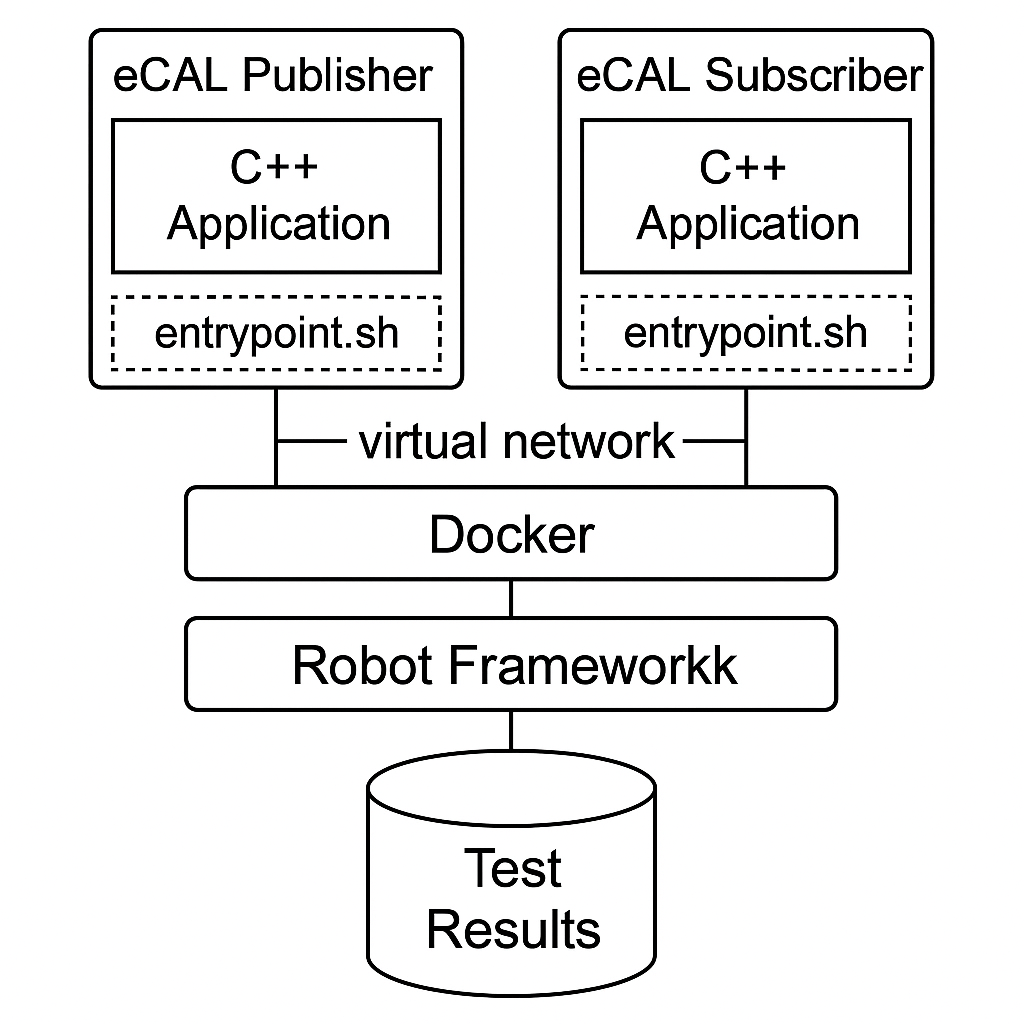
\includegraphics[width=0.72\textwidth]{Images/test_architecture_diagram.png}
 	\caption{Overview of the test environment architecture}
 	\label{fig:test_architecture_diagram}
 \end{figure}
 
The core components of the test architecture are:

\begin{itemize}
	\item \textbf{eCAL Publisher and Subscriber}: Each eCAL node is built as a separate C++ application and runs in its own Docker container. These processes communicate via eCAL using shared topics.
	\item \textbf{Docker Network}: All containers are connected to a common virtual Docker network (e.g., \texttt{ecal\_test\_net}), which enables communication using the selected transport layers.
	\item \textbf{Robot Framework}: The test logic is defined using Robot Framework. It is responsible for starting containers, injecting faults, checking logs, and validating test success criteria.
	\item \textbf{Entrypoint Scripts}: Each container uses an \texttt{entrypoint.sh} script that decides which executable to run (e.g., a publisher, subscriber, or test orchestrator), based on input arguments.
	\item \textbf{eCAL Configuration Files}: Runtime behavior such as communication mode (e.g., UDP vs. SHM) is controlled using \texttt{ecal.yaml} files or configuration overrides in code.
\end{itemize}

The test environment supports all major eCAL communication modes:

\begin{itemize}
	\item \texttt{local\_shm}: Local communication using shared memory.
	\item \texttt{local\_udp}: Local communication using UDP multicast.
	\item \texttt{local\_tcp}: Local communication using TCP.
	\item \texttt{network\_udp}: Network communication using UDP multicast.
	\item \texttt{network\_tcp}: Network communication using TCP.\\
\end{itemize}

This flexible design allows for testing a wide range of scenarios, including those where communication modes must be explicitly selected or changed during runtime. The environment also allows easy simulation of errors, such as killing a process, disconnecting a network, or injecting delays, which are critical for the validation of robustness.

\subsection{Implementation of the Test Infrastructure}

The integration test infrastructure for eCAL was designed to be modular, reusable, and easy to extend. It allows new test cases to be added or removed quickly by following a consistent folder structure and execution pattern. This is particularly useful for one of the most common use cases in test-driven development: adding a new test scenario with minimal overhead.

\vspace{0.5em}
Each component of the infrastructure follows a clear responsibility, which improves maintainability and simplifies debugging. The separation of test logic (e.g., message exchange and failure simulation) and infrastructure logic (e.g., container orchestration) ensures clean design and scalability.

\vspace{1em}
\textbf{1. MyDockerLibrary.py}

\vspace{0.3em}
This custom Python library for Robot Framework provides keywords to manage Docker containers. It offers reusable functions for starting and stopping containers, retrieving logs, checking exit codes, and simulating network disconnections. It abstracts low-level Docker interactions into simple, test-ready keywords.

\vspace{0.5em}
A typical use case is stopping and cleaning up test containers after execution. Listing~\ref{lst:docker_py_stop} shows a simplified implementation of the \texttt{Stop Container} keyword in Python, which handles safe shutdown and removal. Listing~\ref{lst:docker_robot_stop} illustrates how the keyword is used in a Robot Framework test case.

\begin{lstlisting}[style=cppstyle, language=Python, caption={Example keyword implementation in \texttt{MyDockerLibrary.py}}, label={lst:docker_py_stop}, captionpos=b]
 @keyword
  def stop_container(self, name):
    if name in self.containers:
       try:
           self.containers[name].stop()
           self.containers[name].remove()
       except NotFound:
           BuiltIn().log_to_console(f"Container {name} 
           already removed.")
       finally:
           self.containers.pop(name, None)
\end{lstlisting}

\begin{lstlisting}[style=cppstyle, caption={Calling \texttt{Stop Container} in a Robot Framework test}, label={lst:docker_robot_stop}, captionpos=b]
*** Settings ***
 Library           lib/MyDockerLibrary.py	

*** Test Cases ***
 Start Test
  Start Container    my_test_container
  
 ---Test Implementation here---  
 
 Cleanup After Test
  Stop Container    my_test_container
\end{lstlisting}


\vspace{1em}
\textbf{2. GlobalPathsLibrary.py}

\vspace{0.3em}
This library handles dynamic path and tag resolution across all test modules. It defines the active test case, provides access to configuration scripts, and ensures that Docker image names, container labels, and result folders are consistently named and resolved.

\vspace{1em}
\textbf{3. ecal\_config\_helper.h / .cpp}

\vspace{0.3em}
This shared C++ utility is responsible for configuring communication parameters such as transport mode and layer activation. It includes two central helper functions:

\begin{itemize}
	\item \texttt{wait\_for\_subscriber()} – ensures that messages are only published once a subscriber is available (see Listing~\ref{lst:wait_for_subscriber}).
	\item \texttt{setup\_ecal\_configuration()} – configures the desired communication mode (e.g., UDP, TCP, SHM) for each process (see Listing~\ref{lst:setup_ecal}).
\end{itemize}

\begin{lstlisting}[style=cppstyle, caption={Simplified wait\_for\_subscriber logic}, label={lst:wait_for_subscriber}, captionpos=b]
 void wait_for_subscriber(std::string topic){
   while (!has_subscriber(topic)){
     sleep_for(std::chrono::milliseconds(100));
  }
 }
\end{lstlisting}

\begin{lstlisting}[style=cppstyle, caption={Partial example for UDP setup}, label={lst:setup_ecal}, captionpos=b]
 if (mode == "local_udp"){
  config.communication_mode = 
                      eCAL::eCommunicationMode::local;
   if (is_publisher){
      config.publisher.layer_priority_local = 
                       {eCAL::TransportLayer::udp_mc};
   } else {
       config.subscriber.layer.shm.enable = false;
       config.subscriber.layer.udp.enable = true;
       config.subscriber.layer.tcp.enable = false;
    }
  }
\end{lstlisting}

\vspace{1em}
\textbf{5. build\_images.sh}

\vspace{0.3em}
This shell script builds the Docker images required for each test. It invokes CMake to compile the C++ test binaries and packages them together with all dependencies. This ensures consistency between test environments and local development.

\vspace{1em}
\textbf{4. entrypoint.sh}

\vspace{0.3em}
This is the entry script executed inside each container. It uses the given arguments (e.g., role: publisher or subscriber) to launch the correct binary with matching configuration. It also supports scenarios where both publisher and subscriber or multiple binarys are launched together inside the same container.

\vspace{1em}
The infrastructure enables consistent and isolated execution across all test cases while remaining flexible enough to simulate failures, delays, or disconnects. New modes or roles can be added without modifying the core infrastructure.

\subsection{Test Case Design}

This section presents selected integration test cases that were implemented to validate the core behaviors of the eCAL middleware. The tests are executed using Robot Framework and Docker-based containers and make use of the infrastructure described in Section~5.2. Each test focuses on a specific aspect of publisher-subscriber communication and follows a consistent structure.

\vspace{1em}
For every test case, the objective, execution steps, and success criteria are described. In addition, code examples are provided to illustrate important implementation details, such as how publishers and subscribers are configured and how messages are processed. Each test case ends with a short evaluation, which reflects on the observed behavior and explains how the results contribute to the overall test strategy.

\vspace{1em}
\subsubsection{Test Case 1: Publisher to Subscriber Communication}

\textbf{Objective:}

\vspace{0.4em}
Ensure that a message published by a single publisher is reliably received by a single subscriber using a specific transport layer (e.g., shared memory, TCP or UDP) (see Table~\ref{tab:basic_comm_test}).

\vspace{0.5em}
\textbf{Execution:}
\begin{itemize}
	\item In local modes (e.g., \texttt{local shm}, \texttt{local udp}), the publisher and subscriber run inside a single container.
	\item In network modes (e.g., \texttt{network udp}, \texttt{network tcp}), the publisher and subscriber run in separate containers connected via a Docker network.
	\item The publisher sends a small binary payload of value \texttt{42} (repeated) and logs each send event.
	\item The subscriber listens on the topic, logs received values, and exits successfully if the expected messages where received within the timeout window.
\end{itemize}

\textbf{Success Criteria:}
\begin{itemize}
	\item Subscriber receives 100\,\% of all messages sent.
	\item No crashes or communication timeouts occur.
	\item The subscriber exits with return code \texttt{0}.
\end{itemize}

\begin{table}[H]
	\centering
	\begin{tabular}{@{}llll@{}}
		\toprule
		\textbf{Component} & \textbf{Role} & \textbf{Transport Mode} & \textbf{Payload} \\
		\midrule
		basic\_pub  & Publisher  & All Modes  & \texttt{0x2A} (42) \\
		basic\_sub  & Subscriber & All Modes  & 42 \\
		\bottomrule
	\end{tabular}
	\caption{Configuration for Basic Communication Test}
	\captionsetup{position=bottom}
	\label{tab:basic_comm_test}
\end{table}


\textbf{Code Examples:}

\vspace{0.4em}
To illustrate key aspects of the basic communication test, the following code excerpts highlight how the publisher and subscriber are implemented.

\vspace{1em}
The publisher creates a binary buffer of size 10 where each byte is set to \texttt{0x2A} (decimal 42). This value is used consistently across all test scenarios to simplify result verification (see Listing \ref{lst:basic_pub_send}).

\vspace{1em}
The subscriber callback reads the first byte of the received buffer and casts it to an integer. This ensures that the payload can be easily validated (see Listing \ref{lst:basic_sub_receive}).
\vspace{0.5em}

\begin{lstlisting}[style=cppstyle, caption={Binary buffer with value 42 used by the publisher}, label={lst:basic_pub_send}, captionpos=b]
	std::vector<unsigned char> buffer(10, 42);
	pub.Send(buffer.data(), buffer.size());
\end{lstlisting}

\begin{lstlisting}[style=cppstyle, caption={Extracting first byte from the received message in subscriber}, label={lst:basic_sub_receive}, captionpos=b]
	int value = static_cast<int>(
	static_cast<const unsigned char*>(data_.buffer)[0]
	);
\end{lstlisting}

\begin{lstlisting}[style=cppstyle, caption={Argument setup using TCLAP in both publisher and subscriber}, label={lst:tclap_basic}, captionpos=b]
 TCLAP::ValueArg<std::string> mode_arg(
 "m", "mode", "Transport mode", true, "", "string");
 
 TCLAP::ValueArg<std::string> topic_arg(
 "t", "topic", "Topic name", false, "test_topic", "string");
 
 TCLAP::ValueArg<std::string> name_arg(
 "n", "name", "eCAL node name", false, "pub_test", "string");
 
 TCLAP::ValueArg<int> count_arg(
 "c", "count", "Number of messages", false, 3, "int");
 
 TCLAP::ValueArg<int> delay_arg(
 "d", "delay", "Delay between sends", false, 1000, "int");
\end{lstlisting}

\vspace{0.4em}
The configuration with TLCAP in Listing \ref{lst:tclap_basic} allows full flexibility for running the same binary with different roles and transport modes. The \texttt{--mode} parameter (e.g., \texttt{local\_tcp}) enables switching between eCAL transport layers without modifying the code. The use of TCP is especially useful for tests that simulate network scenarios across Docker containers, where shared memory is not apply able.

\vspace{1em}

\textbf{Evaluation:}

\vspace{0.4em}
This basic test confirms that eCAL reliably delivers messages across all supported transport modes under ideal conditions. The results show that communication remains consistent in both local and networked setups, provided the configuration parameters are correctly applied. This test serves as the foundation for more advanced scenarios such as crash handling, message validation, or multi-topic communication.


\vspace{1em}
\vspace{1em}
\subsubsection{Test Case 2: Multiple Publishers and Subscribers}

\textbf{Objective:}

\vspace{0.4em}
Verify that multiple publishers can send distinct payloads on the same topic and that multiple subscribers can receive both streams reliably.

\vspace{0.5em}
\textbf{Execution:}
\begin{itemize}
	\item Two publishers send different payloads (42 and 43) on the same topic.
	\item Two subscribers listen to the same topic and count how many messages they receive for each value.
	\item All four nodes run either in a single container (local mode) or separate containers connected via Docker network (network mode).
\end{itemize}

\textbf{Success Criteria:}
\begin{itemize}
	\item Each subscriber receives 100\,\% of the messages from both publishers.
	\item No crash or message loss occurs during transmission.
	\item All containers exit with return code \texttt{0}.
\end{itemize}

\begin{table}[H]
	\centering
	\begin{tabular}{@{}llll@{}}
		\toprule
		\textbf{Component}     & \textbf{Role}    & \textbf{Transport Mode} & \textbf{Payload} \\
		\midrule
		multi\_publisher       & Publisher        & All Modes               & \texttt{0x2B} (43) \\
		multi\_publisher2      & Publisher        & All Modes               & \texttt{0x2A} (42) \\
		multi\_subscriber      & Subscriber       & All Modes               & Both              \\
		multi\_subscriber2     & Subscriber       & All Modes               & Both              \\
		\bottomrule
	\end{tabular}
	\caption{Configuration for Multi-Publisher and Multi-Subscriber Test}
	\label{tab:multi_pub_sub_test}
\end{table}

\textbf{Code Examples:}
\vspace{0.4em}

Listing~\ref{lst:multi_pub1_send} shows how \texttt{multi\_publisher} sends a binary payload containing value 43. Listing~\ref{lst:multi_pub2_send} illustrates the second publisher, which uses value 42. Both publishers send 15 messages with a 1000\,ms delay between sends.
\vspace{0.5em}
\begin{lstlisting}[style=cppstyle, caption={Publisher 1 sends 0x2B (43)}, label={lst:multi_pub1_send}, captionpos=b]
 std::vector<unsigned char> buffer(10, 43);
 pub.Send(buffer.data(), buffer.size());
\end{lstlisting}
\vspace{0.5em}
\begin{lstlisting}[style=cppstyle, caption={Publisher 2 sends 0x2A (42)}, label={lst:multi_pub2_send}, captionpos=b]
 std::vector<unsigned char> buffer(10, 42);
 pub.Send(buffer.data(), buffer.size());
\end{lstlisting}

Each subscriber uses a callback function that increments counters depending on the first byte received. The values 42 and 43 are tracked separately (see Listing~\ref{lst:multi_sub_receive}).
\vspace{0.5em}
\begin{lstlisting}[style=cppstyle, caption={Subscriber callback counting 42 and 43}, label={lst:multi_sub_receive}, captionpos=b]
 if (value == 42) ++count_42;
 if (value == 43) ++count_43;
\end{lstlisting}

\vspace{0.5em}
\textbf{Evaluation:}

\vspace{0.4em}
This test confirms that eCAL supports N:N communication over a shared topic. Both subscribers successfully received messages from both publishers in all tested transport modes. This demonstrates the middleware's ability to handle concurrent sources and destinations. This is a critical feature for scenarios involving aggregation, monitoring, or distributed decision-making.

\vspace{1em}
From a combinatorial perspective, a complete evaluation of the publish-subscribe model would require testing all communication patterns: one-to-one (1:1), one-to-many (1:N), many-to-one (N:1), and many-to-many (N:N). In practice, however, N:N scenarios inherently cover the functional aspects of both 1:N and N:1 communication patterns. This is because every N:N test includes multiple publishers and subscribers and therefore implicitly verifies the correctness of message delivery from one to many (1:N) and from many to one (N:1) within the same execution.

\vspace{1em}
By implementing N:N tests across all five eCAL transport modes (\texttt{local\_shm}, \texttt{local\_udp}, \texttt{local\_tcp}, \texttt{network\_udp}, \texttt{network\_tcp}), we effectively validate the core functionality and robustness of the middleware under realistic and complex conditions. This strategic reduction in test permutations allows for efficient validation without sacrificing coverage.

\vspace{1em}
\vspace{1em}
\subsubsection{Test Case 3: Publisher Crash During Transmission}

\textbf{Objective:} 

\vspace{0.4em}
Evaluate the system's resilience when one publisher crashes mid-transmission, and ensure that the subscriber still receives messages from the remaining active publisher.

\vspace{0.5em}
\textbf{Execution:}
\begin{itemize}
	\item Two publishers are started: one sends \texttt{42} and crashes after 10 messages, the other sends \texttt{43} continuously.
	\item One subscriber is launched to receive messages from both.
	\item The test runs in all communication modes (local and network).
	\item The subscriber counts messages from both publishers and exits after a fixed timeout.
\end{itemize}

\textbf{Success Criteria:}
\begin{itemize}
	\item The subscriber receives at least 25 messages with value \texttt{43}.
	\item The number of \texttt{42} messages is below the crash threshold (between 5 and 11).
	\item The subscriber exits with return code \texttt{0}.
\end{itemize}

\begin{table}[H]
	\centering
	\begin{tabular}{@{}llll@{}}
		\toprule
		\textbf{Component} & \textbf{Role}     & \textbf{Transport Mode} & \textbf{Payload} \\
		\midrule
		crash\_pub         & Publisher         & All Modes               & \texttt{0x2A} (42) \\
		test\_pub          & Publisher         & All Modes               & \texttt{0x2B} (43) \\
		test\_sub          & Subscriber        & All Modes               & 42 + 43 \\
		\bottomrule
	\end{tabular}
	\caption{Configuration for Crash Resilience Test}
	\label{tab:crash_resilience}
\end{table}

\vspace{0.5em}

\textbf{Code Examples:}

\vspace{0.4em}
The crashing publisher sends a few messages and then exits by calling \texttt{std::abort()}, simulating a runtime failure (Listing~\ref{lst:crash_pub_send}). Meanwhile, the test publisher continues normal operation (Listing~\ref{lst:test_pub_send}).

\vspace{0.5em}
\begin{lstlisting}[style=cppstyle, caption={Crash publisher sends and exits after 10 messages}, label={lst:crash_pub_send}, captionpos=b]
 for (int i = 0; i < total_arg.getValue(); ++i){
  pub.Send(buf.data(), buf.size());
  sleep_for(delay_ms);
  if (i == crash_at_arg.getValue()){
   std::abort();  // Simulate crash
  }
 }
\end{lstlisting}
\vspace{0.5em}
\begin{lstlisting}[style=cppstyle, caption={Resilient publisher continues sending messages}, label={lst:test_pub_send}, captionpos=b]
 for (int i = 0; i < count && eCAL::Ok(); ++i){
  pub.Send(buffer.data(), buffer.size());
  sleep_for(delay_ms);
 }
\end{lstlisting}

The subscriber counts received values and returns 0 only if enough \texttt{43} values are seen and no unexpected continuation from the crashed publisher occurs (Listing~\ref{lst:crash_sub_eval}).

\vspace{0.5em}
\begin{lstlisting}[style=cppstyle, caption={Subscriber decision logic}, label={lst:crash_sub_eval}, captionpos=b]
 if (count_43 >= 25 && count_42 < 11 && count_42 > 4){
   return 0; // Success: resilient communication
 }else{
   return 1; // Failure: not enough or unexpected data
 }
\end{lstlisting}

\vspace{0.5em}

\newpage
\textbf{Evaluation:}

This test demonstrates that eCAL remains fully functional and continues to deliver messages even when one of the publishers crashes unexpectedly. The second publisher, which sends payload \texttt{43}, continues to operate without interruption. This confirms that the failure of one communication node does not affect the functionality of others. The test was executed in all supported eCAL transport modes, showing that this reliability is consistent regardless of the communication layer.

\vspace{1em}

The use of a crash publisher simulates real-world process failures, and the test verifies that message delivery remains uninterrupted. By comparing the message counts, the system ensures that no "phantom" messages are received after the crash point. This approach can be used as a template for testing fault tolerance in distributed IPC systems.

\vspace{1em}
\subsubsection{Test Case 4: Subscriber Crash During Reception}

\textbf{Objective:} \\
Verify that the communication remains stable even when one subscriber crashes while receiving large messages.

\vspace{0.5em}
\textbf{Execution:}
\begin{itemize}
	\item A \texttt{large\_publisher} sends three large messages (each about 50\,MB) on the same topic.
	\item One \texttt{crash\_subscriber} is configured to crash after a short time during message reception.
	\item One \texttt{test\_subscriber} continues running and should receive all messages correctly.
	\item The test is executed in all supported eCAL transport modes, except for local UDP which cannot handle large messages.
	\item A special variant uses SHM with \texttt{zero\_copy\_mode = true} to verify robustness of shared memory access.
\end{itemize}

\textbf{Success Criteria:}
\begin{itemize}
	\item The stable subscriber exits with return code \texttt{0} and logs successful message reception.
	\item The crashing subscriber terminates due to a simulated failure after a few seconds.
	\item The publisher completes message delivery without interruption or failure.
	\item In SHM mode with Zero-Copy, shared memory corruption or deadlocks must not occur.
\end{itemize}

\begin{table}[H]
	\centering
	\begin{tabular}{@{}llll@{}}
		\toprule
		\textbf{Component} & \textbf{Role}       & \textbf{Transport Mode} & \textbf{Payload} \\
		\midrule
		large\_publisher   & Publisher           & All Modes               & $\sim$50\,MB     \\
		crash\_subscriber  & Subscriber (crash)  & All Modes               & $\sim$50\,MB     \\
		test\_subscriber   & Subscriber (stable) & All Modes               & $\sim$50\,MB     \\
		\bottomrule
	\end{tabular}
	\caption{Configuration for Crash During Reception Test}
	\label{tab:sub_crash_receive}
\end{table}

\vspace{0.5em}
\textbf{Code Example:}

The crashing subscriber aborts its process intentionally after two seconds of runtime if it receives any message (see Listing~\ref{lst:sub_crash_logic}).

\begin{lstlisting}[style=cppstyle, caption={Crash condition inside subscriber receive callback}, label={lst:sub_crash_logic}, captionpos=b]
 void OnReceive(
    const eCAL::STopicId&, const eCAL::SDataTypeInformation&,
    const eCAL::SReceiveCallbackData& data_)
 {
  std::cout << "[Crash_Sub] Received " 
  << data_.buffer_size << " bytes\n";
    		
  if (elapsedtime >= 2) {
   std::cerr << "[Crash_Sub] Simulating crash after 2 sec";
   std::abort();
  }
 }

\end{lstlisting}

To simulate high-throughput conditions, the publisher sends three 50\,MB messages and logs each transmission result (see Listing~\ref{lst:large_pub_send}).

\begin{lstlisting}[style=cppstyle, caption={Large message publisher with send confirmation}, label={lst:large_pub_send}, captionpos=b]
 std::string buffer(50L * 1024L * 1024L, 'X');
 for (int i = 0; i < count; ++i){
   bool sent = pub.Send(buffer.data(), buffer.size());
   std::cout << "[Publisher] Send result: " 
             << (sent ? "pass" : "fail");
 }
\end{lstlisting}

\vspace{0.5em}

\newpage
\textbf{Evaluation:}

\vspace{0.4em}
This test confirms that eCAL maintains stable communication even when a subscriber crashes during the reception of a large message. In all tested configurations except the Zero-Copy SHM variant, the system behaved as expected: the publisher completed its transmission successfully, and the stable subscriber received all messages without interruption. The crash was isolated to the failing subscriber, indicating proper error containment and robustness of the communication layer.

\vspace{1em}
The variant using Zero-Copy in Shared Memory mode highlighted a specific weakness in fault isolation. In Zero-Copy mode, the publisher shares direct memory access with subscribers, which eliminates the need for memory copying and significantly improves performance in high-throughput scenarios. However, this optimization also introduces a stronger coupling between processes at the memory level.

\vspace{1em}
If a subscriber crashes while holding a pointer to shared memory, the publisher (or other subscribers) may experience access violations, resource locks, or inconsistent memory states. This was observed during the test: although the publisher attempted to continue sending data, the shared memory segment could no longer be accessed safely once the crashing subscriber aborted during callback execution. 

\vspace{1em}
Therefore, while Zero-Copy SHM offers performance advantages, it requires careful handling in fault-tolerant systems. Mechanisms such as memory fencing, process monitoring, or fallback copy modes should be considered if system resilience is a priority.

\vspace{1em}
In conclusion, this test underscores both the reliability of eCAL in standard SHM, TCP, and UDP scenarios and the current limitations when using Zero-Copy SHM without additional safeguards. Future testing or deployment scenarios should carefully consider the trade-off between performance and fault tolerance when using advanced features like Zero-Copy.

\newpage

\vspace{1em}
\subsubsection{Test Case 5: Network Failure Simulation}

TODO

\newpage
\subsection{Handling of Edge Cases}

In addition to testing typical communication flows, the test infrastructure also covers a variety of edge cases that may occur in distributed systems. These cases are particularly important for evaluating the robustness and fault tolerance of the eCAL middleware under non-ideal conditions.

\vspace{0.5em}
The following categories of edge cases are addressed:

\begin{itemize}
	\item \textbf{Timing jitter and delays} \\
	To simulate unstable timing behavior, artificial delays are introduced using \texttt{sleep} call to manipulate network latency. This helps verify whether eCAL nodes can still synchronize and communicate reliably under varying timing conditions.
	
	\item \textbf{Crash simulation} \\
	Component failures are simulated by forcefully stopping or disconnecting Docker containers. This reflects real-world scenarios such as sudden application crashes or network cable unplugging. The system’s ability to recover, reconnect, or log the error is then observed.
	
	\item \textbf{Missing communication partners} \\
	In some tests, publishers are started without any active subscribers. This tests whether the publisher behaves correctly in absence of receivers, without blocking or generating errors.
\end{itemize}

\vspace{0.5em}
To evaluate the outcome of these tests, different observation methods are applied:

\begin{itemize}
	\item \textbf{Exit code monitoring} \\
	Each container returns an exit code upon completion. A code of \texttt{0} indicates successful execution, while non-zero values signal unexpected behavior or test failure.
	
	\item \textbf{Log analysis} \\
	Container logs are collected and printed by the Robot Framework. These logs include important debug messages and warnings generated by the eCAL nodes and the test logic.
	
	\item \textbf{Payload validation} \\
	In several tests, the payload value is checked directly to verify that messages were received correctly and from the expected source.
\end{itemize}

This structured approach to handling edge cases ensures that both functional correctness and system reliability are fully tested under the most challenging conditions.


\subsection{Automation and Repeatability}

One of the main goals of the integration test design is to ensure that all tests can be executed in a fully automated and repeatable way. Automation is essential for running regression tests frequently and reliably—especially when integrating the tests into CI/CD pipelines.

\vspace{0.9em}
The tests are executed using Robot Framework and can be triggered with a single command:

\begin{verbatim}
	robot --outputdir results network_crash.robot
\end{verbatim}

\vspace{0.5em}
This command runs the specified test and stores the output files in the \texttt{results} directory. The following artifacts are automatically generated after each run:

\begin{itemize}
	\item \textbf{log.html} – Detailed step-by-step execution log with console output
	\item \textbf{report.html} – Summary report with pass/fail statistics
	\item \textbf{output.xml} – Raw result data (used for machine-readable processing or CI systems)
\end{itemize}

\vspace{0.5em}
The simplicity and structure of this test approach makes it well suited for integration into CI/CD systems such as GitHub Actions or GitLab CI. These systems can be configured to run the test suite automatically after every commit or pull request, ensuring that communication functionality remains stable even during ongoing development.

\vspace{0.9em}
Furthermore, since Docker is used for test isolation, the tests are highly portable and can run in local development environments, on build servers, or in virtualized testing infrastructure with minimal setup.

\newpage
\subsection{Summary}

This chapter presented the design, implementation, and execution of a modular integration test system for the eCAL middleware. By combining Docker-based process isolation with the flexible automation capabilities of Robot Framework, it was possible to validate key properties of publish-subscribe communication in a controlled and reproducible environment.

\vspace{1em}
The selected test cases focused on core functionalities such as reliable message delivery, multi-node communication, and fault tolerance under crash or failure conditions. Most scenarios were tested across all five supported eCAL transport modes, these are shared memory (SHM), UDP, and TCP in both local and network configurations. This ensured broad coverage of both common and edge-case communication patterns.

\vspace{1em}
Code examples demonstrated how publishers, subscribers, and test logic are implemented and configured, while structured success criteria and exit codes provided clear validation of expected behavior. The test infrastructure also proved effective in simulating failure scenarios such as process crashes and message loss, confirming the robustness and resilience of the eCAL middleware.

\vspace{1em}
A notable insight from these tests is the performance–resilience trade-off introduced by advanced features like Zero-Copy SHM. While this mode improves throughput by eliminating memory copies, it also increases inter-process coupling and may compromise fault isolation if a subscriber crashes during message access. Future deployments should carefully assess whether the performance benefits of Zero-Copy justify its potential stability risks.

\vspace{1em}
The framework is already equipped to be extended with further test categories. For example, future work could include RPC-based communication, service availability tests, and metrics such as round-trip time. Moreover, integration into CI/CD pipelines would enable automatic regression testing during development and deployment.

\vspace{1em}
In conclusion, the developed test system successfully demonstrates how integration tests can be used not only for functional verification but also to explore system behavior under realistic and adverse conditions. It provides a solid foundation for continuous validation of middleware functionality in research, development, and production contexts.



\selectlanguage{english}
\clearpage
\section{Conclusion and Outlook (TODO)}
// TODO
\newpage
\printbibliography[heading=bibintoc]
\end{document}


